As already mentioned, there have been 3 independent earthquakes, as could be 
seen in Figure~\ref{fig:eq_start_heat}: Apr 6th 2:00~PM, Apr 8th 7:00~AM and Apr 
9th 3:00~PM, approximately. Those two last earthquakes are emphasized in
Figure~\ref{fig:eq_2_3_heat}.

\begin{figure}[!h]
    \centering
    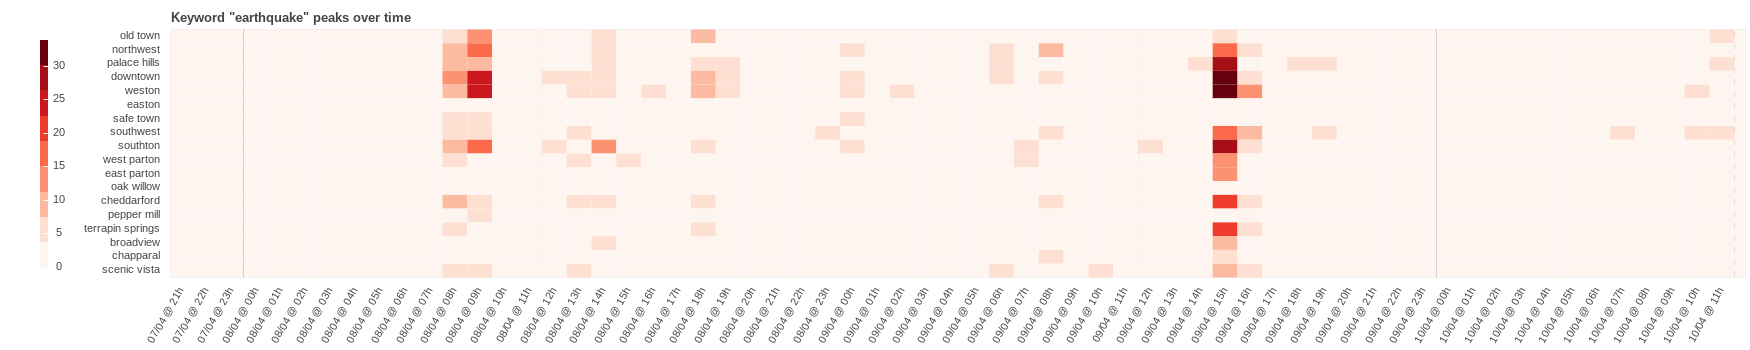
\includegraphics[width=1.00\textwidth]{figs/q2/eq_2_3_heat}
    \caption{Heatmap for the two last earquakes using keywords related to the
    word ``earthquake''.}
    \label{fig:eq_2_3_heat}
\end{figure}

\begin{figure}[!h]
    \centering
    \begin{subfigure}[!h]{0.96\textwidth}
        \centering
        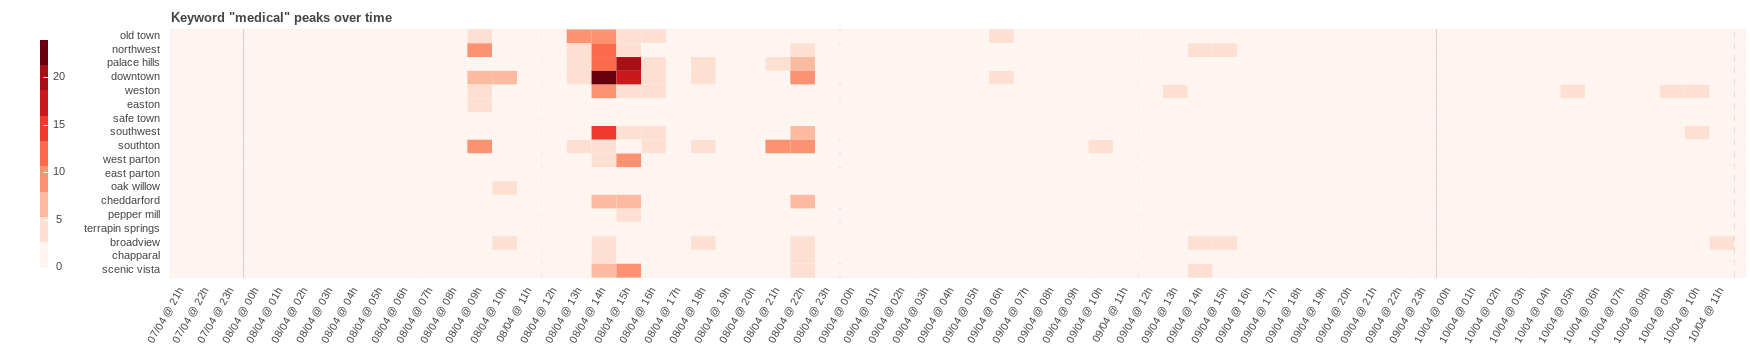
\includegraphics[width=1.00\textwidth]{figs/q2/medical_2_3_heat.png}
        \caption{Medical}
        \label{fig:medical_2_3_heat}
    \end{subfigure}
    \begin{subfigure}[!h]{0.96\textwidth}
        \centering
        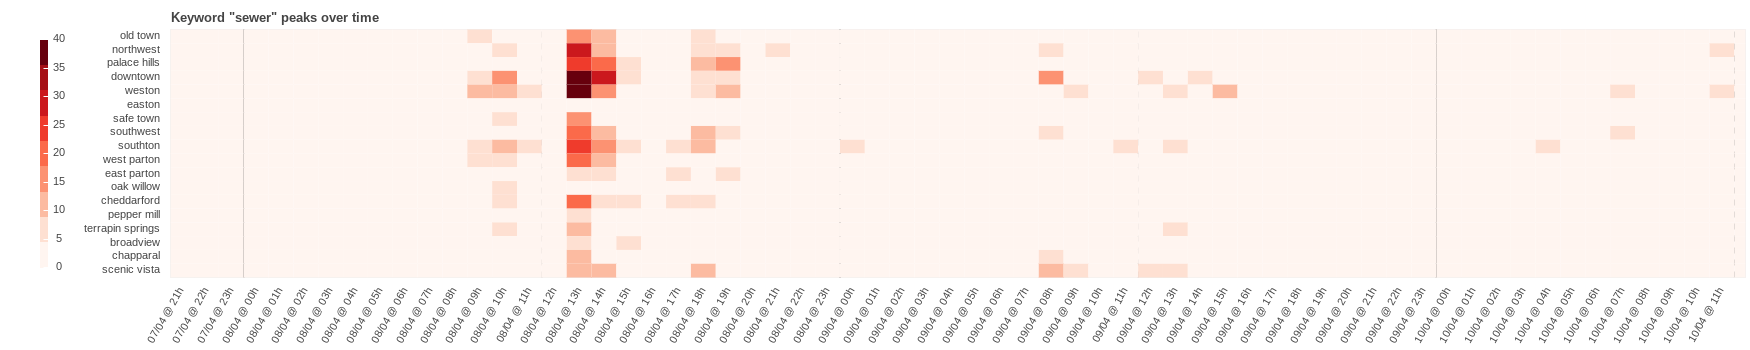
\includegraphics[width=1.00\textwidth]{figs/q2/sewer_2_3_heat.png}
        \caption{Sewer and water}
        \label{fig:sewer_2_3_heat}
    \end{subfigure}
    \begin{subfigure}[!h]{0.96\textwidth}
        \centering
        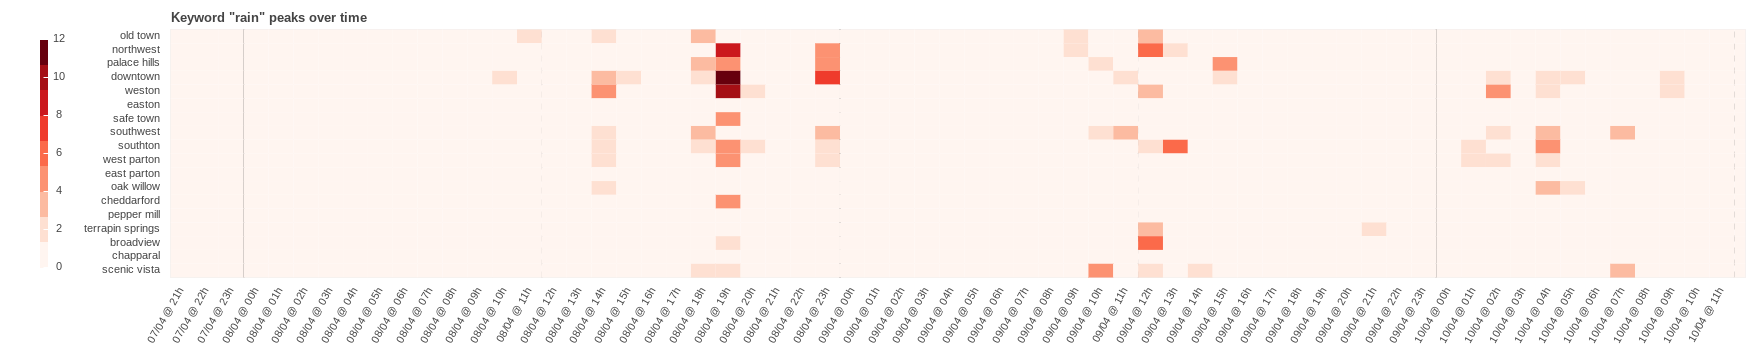
\includegraphics[width=1.00\textwidth]{figs/q2/rain_2_3_heat.png}
        \caption{Rain}
        \label{fig:rain_2_3_heat}
    \end{subfigure}
    \begin{subfigure}[!h]{0.96\textwidth}
        \centering
        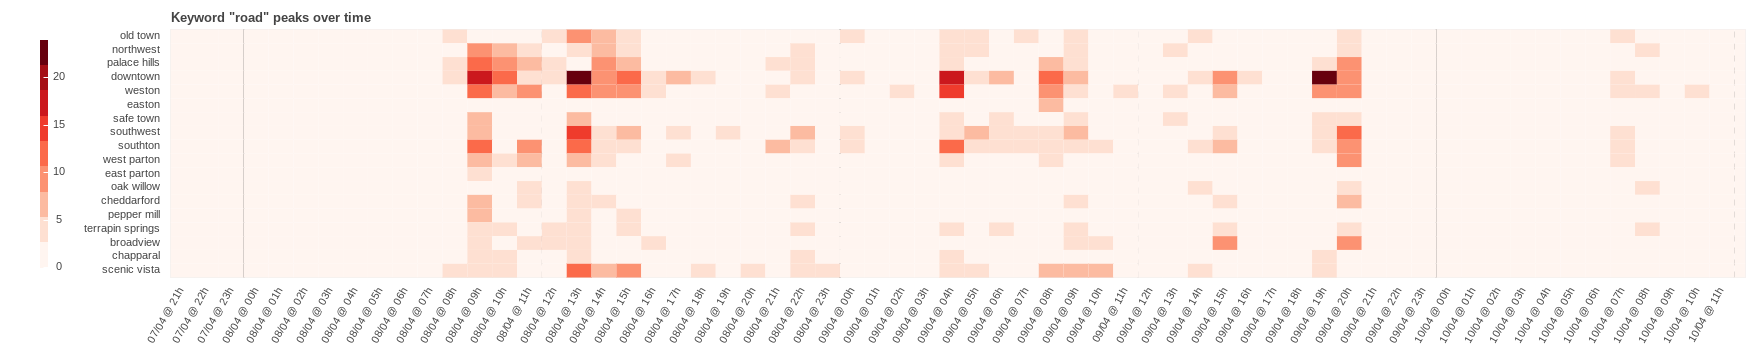
\includegraphics[width=1.00\textwidth]{figs/q2/road_2_3_heat.png}
        \caption{Roads and Bridges}
        \label{fig:roads_2_3_heat}
    \end{subfigure}
    \begin{subfigure}[!h]{0.96\textwidth}
        \centering
        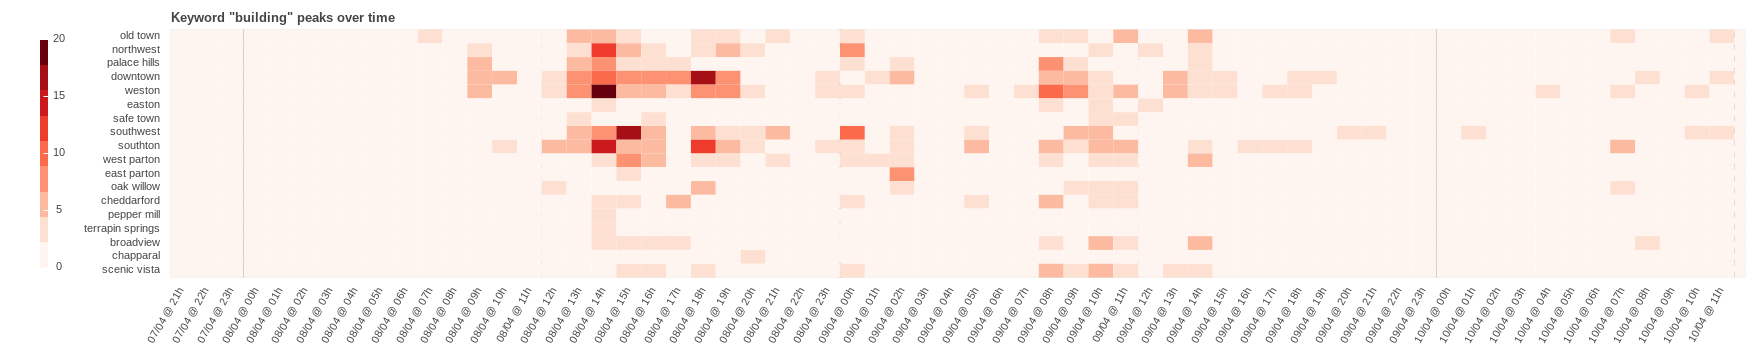
\includegraphics[width=1.00\textwidth]{figs/q2/build_2_3_heat.png}
        \caption{Building}
        \label{fig:building_2_3_heat}
    \end{subfigure}
    \begin{subfigure}[!h]{0.96\textwidth}
        \centering
        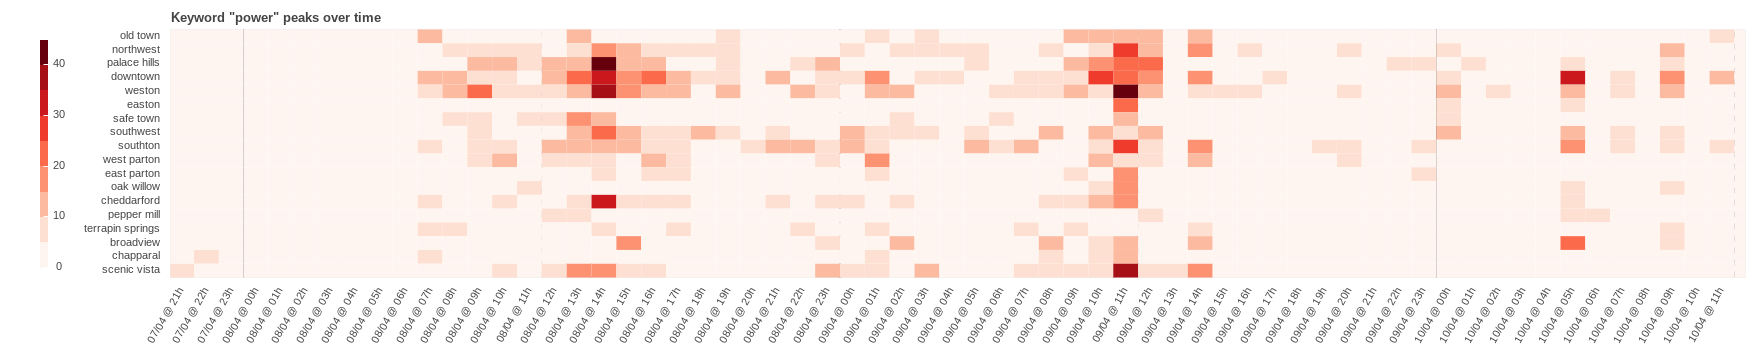
\includegraphics[width=1.00\textwidth]{figs/q2/power_2_3_heat.png}
        \caption{Power}
        \label{fig:power_2_3_heat}
    \end{subfigure}
    \caption{Heatmap of conditions for the two last earthquakes}
    \label{fig:eq_cond_2_3_heat}
\end{figure}

By looking at the heatmap of Figure~\ref{fig:eq_cond_2_3_heat} for each
keyword, it can be seen that the damaged inflicted by the
second earthquake was greater than both first and second ones.

Suggestions for re-allocation of city resources are detailed as follows:   

\begin{itemize}                                                                  
     \item \emph{Medical:} At least 12 hours before 9:00 AM of April 8th, there was no ocurrances regarding
medical keywords. 
\begin{itemize} 
\item On April 8th from 9:00 PM to 10:59 PM, the second earthquake
time, there have been casualties on multiple locations
but we would prioritize the darker colored ones according to the heatmap of Figure 8a:
Northwest, Southton and Downtown. First, a rescue crew must be sent to Northwest
and Southton between     
     9:00~AM and 9:59~AM. Then, from 9:00~AM to 9:59~AM, for being geographically close a crew must be realocated to
Downtown. 

\item Again, between 12:00 PM and 13:00 PM there have been no medical ocurrances but from 13:00 PM
to 16:00 PM, the number of ocurrances increased significantly and affected
almost all neighbourhoods except Safetown and Terrapin Springs. Accordingly, we
would prioritize the dark-red-colored ones, Downtown and Palace Hills, sending
rescue team from 14:00~PM to 15:00~PM for both neighbourhoods.  

\item On following hours after that peak in ocurrances, there have been only sporadic
requests that could be solved by sending small units to individual locations.
 \end{itemize} 
\item \emph{Sewer and water:} A crew must be sent only to Weston between 4:00~PM and 4:59~PM.                                                          
     \smallskip                                                                   
     \item \emph{rain}: Issues have occurred in Pepper Mill, \textbf{Terrapin    
     Springs}, \textbf{Broadview}, Chapparal, \textbf{Southton}, \textbf{Old      
     Town} and Scenic Vista, but we'll consider only the locations                
     highlighted in bold because they have hospitals.                             
     \begin{itemize}                                                              
         \item A crew must be sent to Terrapin Springs between 3:00~PM and        
         3:59~PM. Broadview also has a power demand at this time interval but the 
         tweet frequency is much lower considering the five-hour period.                           \item Two crews must be sent to Old Town and Southton between 4:00~PM    
         and 4:59~PM.                                                             
         \item Lastly, the crew from Terrapin Springs can be reallocated to                Chapparal between 5:00~PM and 5:59~PM. Although Chapparal does not have  
         hospitals, it has been nearly two hours with electrical issues.          
     \end{itemize}                                                                
     \item \emph{R}: A crew must be sent to Southton only   
     because there have been small issues in Weston, Southton and Downtown, and   
     therefore Southton is geographically in the middle of such neighbourhoods.   
 \end{itemize}   

\begin{figure}[!h]
    \centering
    \begin{subfigure}[!h]{0.98\textwidth}
        \centering
        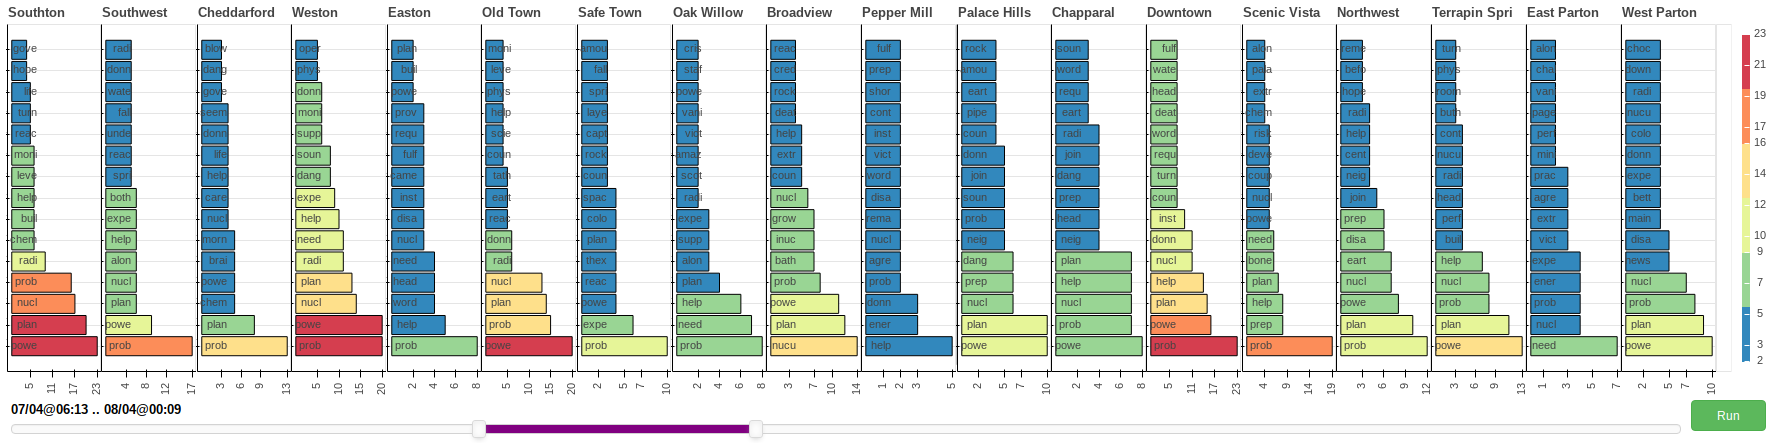
\includegraphics[width=1.00\textwidth]{figs/q2/eq_2_hbar.png}
        \caption{Bar chart for the second earthquake in a 18h time interval from
        Apr 7th at 6:00~PM to Apr 8th at 12:00~AM.}
        \label{fig:eq_2_hbar}
    \end{subfigure}
    \begin{subfigure}[!h]{0.98\textwidth}
        \centering
        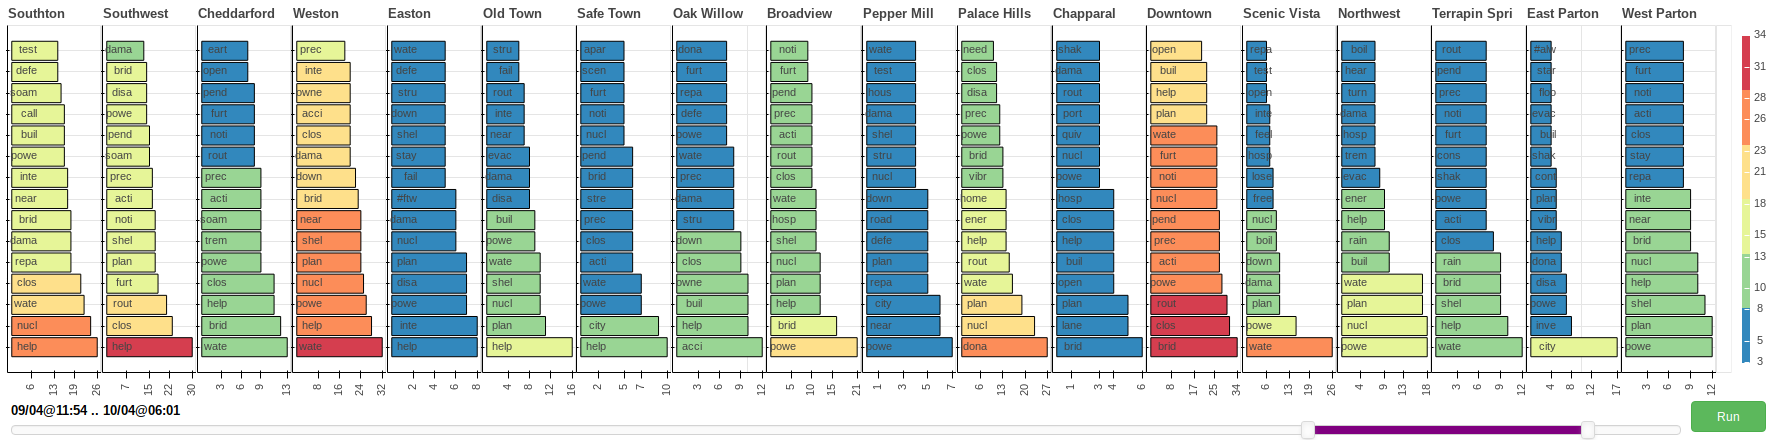
\includegraphics[width=1.00\textwidth]{figs/q2/eq_3_hbar.png}
        \caption{Bar chart for the third earthquake in a 18h time interval from
        Apr 9th at 12:00~PM to Apr 10th at 6:00~AM.}
        \label{fig:eq_3_hbar}
    \end{subfigure}
    \caption{eae}
    \label{fig:eq_2_3_hbar}
\end{figure}

\begin{figure}[!h]
    \centering
    \begin{subfigure}[!h]{0.46\textwidth}
        \centering
        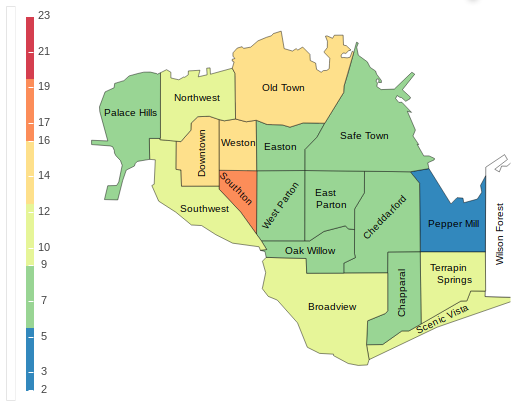
\includegraphics[width=1.00\textwidth]{figs/q2/eq_2_svg.png}
        \caption{Map for the second earthquake. Yellow and orange shades show
        locations where the frequency of tweets is higher. Southton, Downtown,
        Weston and Old Town appear to be, in that order, the neighbourhoods that 
        most need help.}
        \label{fig:eq_2_svg}
    \end{subfigure}
    \hspace{0.75cm}
    \begin{subfigure}[!h]{0.46\textwidth}
        \centering
        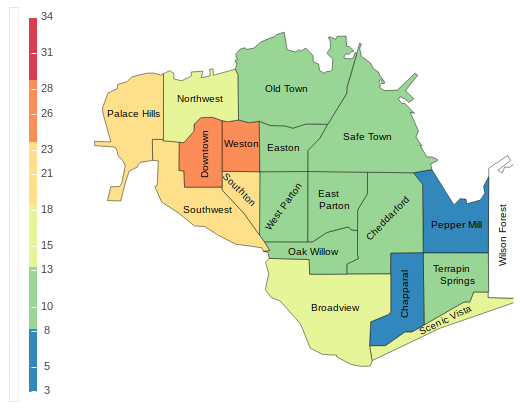
\includegraphics[width=1.00\textwidth]{figs/q2/eq_3_svg.png}
        \caption{Map for the third earthquake. Yellow and orange shades show
        locations where the frequency of tweets is higher. Downtown, Weston,
        Pallace Hills, Southwest, and Southton appear to be, in that order, the 
        neighbourhoods that most need help.}
        \label{fig:eq_3_svg}
    \end{subfigure}
    \caption{St. Himark's SVG maps with blue-to-red colormap for the second and
    third earthquakes.}
    \label{fig:eq_2_3_svg}
\end{figure}

